\documentclass[letterpaper,times]{IONconf/IONconf}

\usepackage{amsmath}
\usepackage{graphicx}
\usepackage{multirow}
\usepackage{float}
\usepackage[ruled,vlined]{algorithm2e}

\title{On SBAS Authentication with OTAR Schemes}
\author{Jason Anderson, Todd Walter, et al.}

\begin{document}

\maketitle

\begin{abstract}
Herein we delineate a complete SBAS authentication scheme, including over-the-air re-keying (``OTAR'').
This scheme appends two new message types (''MT'') to the SBAS scheduler without overburdening the SBAS message schedule or using the Q channel.
We take special care to make our scheme (1) meet the appropriate security requirements to prevent and deter spoofing, (2) compatible with existing cryptographic standards, (3) flexible, expandable, and future proof to different cryptographic and implementation schemes, and (4) backward compatible with legacy receivers.
The scheme requires loose time synchronization between the receiver and the provider.
We assert reasonable requirements on the receiver clock uncertainty, calibration, and startup procedures to prevent spoofing via a GNSS and SBAS replay attack.
This work also discusses the SBAS provider and receiver machine state and startup, including as they apply to aircraft that traverse differing SBAS coverage areas.
We test our scheme with existing SBAS simulation and analysis tools to show better performance against other schemes previously suggested and negligible effects on SBAS availability and continuity requirements.
We also suggest that this scheme would be useful broadly to any bandwidth-limited broadcast-only authentication scheme.
\end{abstract}

\section{Introduction}

In this work, we delineate a complete Satellite-Based Augmentation System (the service itself, ``SBAS'') authentication scheme, including over-the-air re-keying (``OTAR'') and then discuss how this proposed scheme meets necessary security levels and desirable traits to SBAS stakeholders, such as backward compatibility, data efficiency, and quick time to authenticated first fix.
Moreover, it is expandable to additional stakeholder feedback.
This work addresses the full authentication scheme design, including connecting receiver hardware requirements to maintenance schedules, key updates, and scheme maintenance, and uses a full-stack Monte-Carlo SBAS simulation to test and evaluate the scheme's performance.

Satellite-Based Augmentation Systems (the several international systems together, ``SBASs''), such as the United States' Wide-Area Augmentation System (``WAAS'') among other international equivalents, have become integral to the Global Navigation Satellite System (``GNSS'') for civilian aviation use.
International parties that choose to implement an SBAS (each a ``Provider'') use listening stations around their service volume to assess GNSS satellite positioning data and then broadcast those assessments widely via geostationary satellites.
This information includes wide-area GNSS differential corrections and GNSS satellite health and integrity.
Like most GNSS core-constellation signals, the SBAS signal is open and susceptible to spoofing, and with its ubiquitous use in civilian aviation, SBAS should be augmented with spoofing resistant capabilities to ensure continued civilian aviation safety.
The Providers agree to share a common SBAS message standard.
This work pertains to how the SBAS message standard could be augmented to provide an authenticated service resistant to spoofing.

SBAS is primarily a data service.
It broadcasts data that assists GNSS users.
Therefore, appending additional cryptographic data to the SBAS data serves as a natural way to authenticate the SBAS data for civil users.
This would require that SBAS broadcast messages that deliver cryptographic signatures and key values to users.
Using the mathematical primitives underlying cryptographic authentication methods, users would assert that only Provider could have generated the SBAS data and the accompanying authenticating ciphertext.
In this work, we call the authenticating data "signatures", and signatures, together with the associated key data, ``authenticating ciphertext''.
We call this data authenticating ciphertext not because it contains a cipher, but because the data is psuedorandom and not human-readable.
The security of the authenticating ciphertext assumes that (1) Provider exclusively holds certain identifying information secret and (2) there exist no {\em known} efficient algorithms that can generate the authenticating ciphertext without the identifying information held secret.
If the identifying information (e.g., keys) is leaked, that information is called compromised and must be revoked.
If an efficient algorithm is discovered, the scheme is called broken and the associated mathematical primitives must be replaced.

Using cryptographic authentication methods poses certain challenges to SBAS.
The main challenge is delivering the ciphertext via SBAS, given the data-bandwidth constraints.
SBAS authentication security must rely on asymmetric cryptographic algorithm to provide authentication, such as Elliptic Curve Digital Signature Algorithm (``ECDSA'').
Herein, wherever we specify ECDSA, we could use another similar asymmetric cryptographic algorithm (e.g., EC-Schnorr); however, we will specify ECDSA without losing generality for concreteness noting that certain parameters and characteristic security strengths listed here would be different if not using ECDSA.
To meet a standard 128-bit security level, a single signature requires 512-bits, which dwarfs the maximum allowable SBAS data bits per message at 216 bits.
Prior art has suggested using the Quadrature (``Q'') channel to deliver the authenticating ciphertext \cite{other_schemes}; however, those solutions would require power from the current use of the In-phase (``I'') channel.
Using the Q-channel would strain the availability and continuity of SBAS systems at coverage area boundaries, which is undesirable to SBAS stakeholders.
Prior art has suggested using a combination of ECDSA with another algorithm called Timed Efficient Stream Loss Tolerant Authentication (``TESLA'') \cite{Neish_Dissertation} since it provides more efficient use of ciphertext and is loss tolerant.
TESLA uses a delayed-release mechanism to authenticate data with less authenticating ciphertext than that required by ECDSA; however, it requires that Provider and a user be loosely time-synchronized \cite{perrig2005timed}.
SBAS cannot exclusively use TESLA; TESLA must be used in tandem with ECDSA to achieve authentication security.
The relationship between the proposed TESLA-ECDSA scheme can be described as follows: TESLA authenticates the SBAS messages themselves, and ECDSA authenticates SBAS's use of TESLA as periodic {\em maintenance}.
The prior work has specified that TESLA and ECDSA scheme parameters required to achieve authentication; however, it has largely not addressed the maintenance and maintenance requirements, such as how best to OTAR.
This work addresses the main challenge by suggesting a more efficient authentication maintenance scheme without using the Q channel.

Prior art suggested appending a single message type (``MT'') to SBAS for authentication and its maintenance\cite{Neish_Dissertation}.
It suggests that SBAS sends this MT every six messages and that this MT delivers 190-bits of TESLA authentication data and 26-bits for the scheme's maintenance.
While the scheme requires a steep authentication-message delivery frequency, it does not overburden the SBAS MT schedule.
In this work, we modify prior art by appending another MT to SBAS to replace the 26-bits mentioned above dedicated for maintenance.
We design our proposed additional MT to be modular with the exclusive purpose of delivering all authentication ciphertext related to the scheme's maintenance.
This design allows for reasonable time-to-first-authenticated-fix requirements.
It is agnostic to the ECDSA and TESLA scheme parameters; therefore, it requires no changes in the event of cryptographic primitive breakage.
Moreover, it scales well with increases to the security level requirements and is flexible and future-proof to anticipated feedback from Providers and SBAS stakeholders.

To evaluate the proposed method against prior art, we implement a full-stack SBAS simulation of our design by augmenting an existing SBAS simulation tool called Matlab Algorithm Availability Simulation Tool (``MAAST'')\cite{MAAST}.
MAAST has been used to evaluate SBAS design before and provides Monte-Carlo simulation results to evaluate how our design performs under message loss over the WAAS coverage area.
With the tool, we show that our proposed design outperforms Key Performance Indicators (each a ``KPI''), such as time to first authenticated fix, time to authentication per message, and robustness to message loss.

With TESLA's use, Provider and any users must be loosely time-synchronized, which poses an interesting Catch-22 situation since GNSS provides the time.
Therefore, our scheme must also describe its resistance to a Replay Attack.
A Replay Attack is where a spoofer listens and then replays messages at a slightly delayed rate.
After some time, the spoofer-induced time delay allows the spoofer to violate the loosely-time synchronized assumption and break the TESLA scheme.
Prior art has described how a receiver on-board clock could be used to detect such an attack, given clock uncertainty \cite{time_sync_paper}.
This work extends this work by specifying the on-board clock accuracy requirements and maintenance schedules to meet our scheme's security level, and we find those requirements reasonable for SBAS receivers.

\subsection{ECDSA}
ECDSA is a standardized asymmetric authentication protocol.
The protocol specifies a signing function and a verifying function.
Let $n$ be the security level of an instance of the protocol, which linearly describes the required computation to {\em exhaustively} break the instance.
Provider generates a secure random $2n$-bit integer for long-term use as a secret private key.
Provider then derives a $2n$-bit integer from the private key and distributes to receivers as the public key.
Provider uses the signing function, with the secret private key, to derive signatures on messages.
Each signature is a $4n$-bit integer.
Receivers use the verifying function, with the public key and signatures, to assert that the holder of the private key generated the message and signature.
Since the protocol is secure, there is no {\em known} efficient algorithm that can compute the private key given the public key nor compute the signature on a message.
By efficient algorithm, we mean any algorithm that is faster than exhaustive search on the total 2n-bit private key space.
The protocol assumes that the receiver trusts the public key as from Provider.
The protocol is not loss-tolerant: if a single bit of a signature or message is lost, the protocol will fail to verify.

\subsection{TESLA} \label{sec: TESLA intro}

TESLA is an authentication protocol that allows a receiver to authenticate messages from Provider when used in tandem with other asymmetric authentication protocols.
This protocol poses several advantages over a purely asymmetric system relevant to GNSS and SBAS systems.
First, the protocol requires less authenticating ciphertext to authenticate messages from Provider.
Second, the protocol is loss-tolerant.
Third, the receiver authentication computation is less strenuous.
Figure \ref{fig: TESLA Diagram} provides a conceptual diagram of the TESLA description that follows.
Algorithm \ref{alg: TESLA} describes the protocol more concretely.

\begin{figure}
\centering
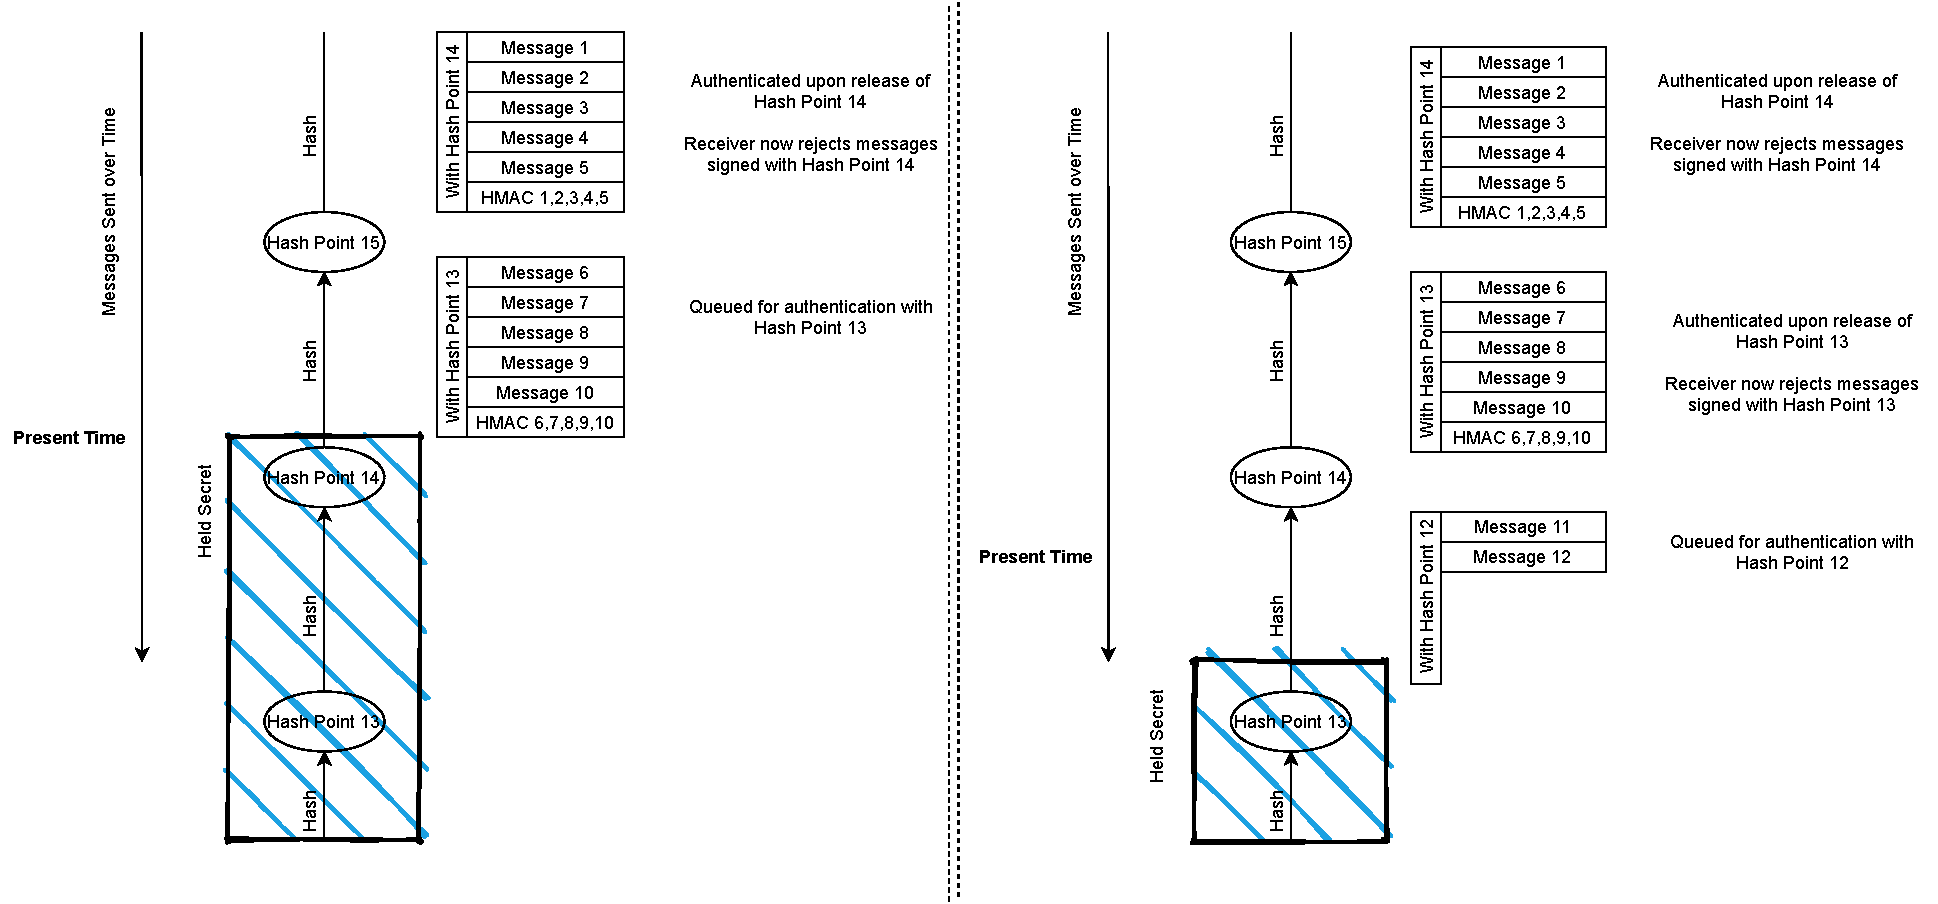
\includegraphics[width=\linewidth]{fig/TESLADiagram.pdf}
\caption{Conceptional diagram of TESLA. The right section of the diagram follows the left section of the diagram in time.}
\label{fig: TESLA Diagram}
\end{figure}

TESLA uses only a single cryptographic primitive: a cryptographically-secure hash function.
In this proposal, we select a salted SHA-256, truncated to 128-bits (herein, the ``Hash Function'' or $\textrm{H}(\cdot)$), so we describe the TESLA protocol concretely using our selection without loss of generality.
We restrict the Hash Function domain to be equivalent to its range: the set of 128-bit integers.
Since the audience of this work are experts in navigation, we use geometric terms {\em path} and {\em point} instead of {\em key chains} and {\em key} and describe TESLA with the geometry of a {\em one-way path}.
Let each 128-bit integer be called a Hash Point, and let a collection of Hash Points {\em consecutively} related via the Hash Function be a Hash Path.
Hash Points further along the Hash Path -not consecutive- are related by repeated application of the Hash Function.
Since the Hash Function is secure, there is no {\em known} efficient algorithm that can compute the input Hash Point to the Hash Function that yields a specific output Hash Point.
Herein, we call that input Hash Point the preimage Hash Point of that output Hash Point.
In other words, it is trivially easy to compute the output Hash Point of the Hash Function given the preimage Hash Point, but one can only use exhaustive search to find any preimage Hash Point.
It is a {\em one-way} path.
The domain of 128-bit integers, together with a randomized 128-bit salt inclusion to the Hash Function, make precomputation attacks (also called Rainbow Table Attacks) infeasible with modern supercomputers because it meets 128-bit security.

To use a Hash Path to authenticate messages via TESLA, Provider computes a Hash Path derived from a {\em random} starting Hash Point and holds that Hash Path secret.
Provider broadcasts the last Hash Point along the Hash Path (herein, the "Hash Path End") together with an ECDSA signature derived therefrom.
Receivers assert the Hash Path End as authenticated with the ECDSA signature.
Provider uses the secret preimage Hash Point to the Hash Path End as a key to send symmetric authentication signatures along with the standard message set.
We propose using keyed-hash message authentication codes that use the Hash Function as its primitive as the signatures (the function, ``HMAC'', and the HMAC signatures themselves, ``HMACs''). 
We will continue to describe the protocol concretely using our selection without loss of generality.
Providers and receivers agree on schedule where Provider will (1) stop using the preimage Hash Point of the Hash Path End to authenticate messages, (2) broadcast that preimage Hash Point for receivers to authenticate messages, and (3) use the next preimage Hash Point along the Hash Path to authenticate new messages.
Once a particular preimage Hash Point is broadcast, receivers cannot accept new signatures received derived therefrom.
Since the HMACs were received when a specific preimage Hash Point was known only to Provider, the messages must have been generated by Provider.
Each time Providers release a Hash Point, Provider moves backward one Hash Point along its secret Hash Path to derive new HMACs.

The authentication security along the Hash Path hinges on (1) the security of the Hash Function and (2) that Provider and receiver are loosely time-synchronized.
Since the Hash Point is known only to Provider when the HMACs were computed, only Provider could have generated those messages.
Provider releases Hash Points on the known schedule provided by the loosely-time-synchronized assumption, and Provider notes that only messages received with the correct signature {\em before} that release can be authenticated.
Given the Hash Function's security, the Hash Point along the Hash Path before the released Hash Point is still secret, and so it becomes the new HMAC key for the next set of messages.

To complete the authenticating security, TESLA must be used in tandem with an asymmetric authentication protocol.
TESLA is secure along the Hash Path length; however, Hash Paths are finite and must be generated periodically.
An asymmetric authentication protocol must sign the Hash Path End, the first Hash Point known to the receiver.
In other words, for every Hash Path generated by Provider, Provider must use an asymmetric signature to ensure authentication security along the entire Hash Path.
Moreover, Provider and receiver must be loosely time-synchronized, which poses a Catch-22 problem since GNSS and SBAS Providers provide the time.
This provokes the question of why use TESLA at all and not just use only an asymmetric protocol.
Later in this work, we will show that using TESLA has better loss-tolerant properties and requires less ciphertext, and the time-synchronization problem can be accounted for.

\section{Proposed Message Definitions} \label{sec: definitions}

This SBAS authentication proposal proposes appending two message types to the schedule (herein, ``MT50'' and ``MT51'').
MT50 is used to authenticate the actual SBAS messages via the TESLA protocol.
MT51 is used to (1) authenticate the Hash Path Ends via ECDSA as Provider uses series of Hash Paths in its standard operation, and (2) to provide over-the-air-rekeying (``OTAR'') and perform system-level maintenance of the cryptographic authentication scheme.
Here follows in this Section \ref{sec: definitions} precise definitions of our proposed SBAS authentication scheme.
Section \ref{sec: methodology} provides explanations and reasoning for our proposed definitions.
While the definitions presenter here are for the L5 signal, given the spare bits remaining in each definition, this scheme will also work for the L1 signal by modifying the preambles.

\subsection{ECDSA Key Structure} \label{sec: ECDSA Key Structure}

We propose a two-level ECDSA key structure, as suggested \cite{Neish_Dissertation}.

Level-1 keys will be 256-bit ECDSA keys managed by the  International Civil Aviation Organization (``ICAO'').
Each level-1 key will be in use for 100 weeks.
ICAO shall compute a large number of level-1 keys for use in the perpetual future and then encrypt each key separately via AES-128 with those encryption keys held secret by ICAO.
ICAO will distribute the AES-ciphertext to receiver manufacturers.
Receivers will come preloaded with the collection of 512-bit public keys, encrypted with 128-bit keys via AES-128.
As level-1 keys expire, ICAO will distribute the keys to decrypt the AES-ciphertext, one at a time, for Provider to distribute.
As the receiver receives the key to decrypt its on-board AES-ciphertext, it will update its current level-1 ECDSA public key.
Each level-1 public key will be a 512-bit integer, and any signature derived therefrom will be a 1024-bit integer.

Level-2 keys will be 128-bit ECDSA keys managed by Provider.
Each level-2 key will be in use for 10 weeks.
For a new level-2 key, Provider will generate a secure-random private ECDSA key and its associated public key.
Provider will submit the new public key to ICAO for a signature from ICAO's current level-1 key.
Provider will then distribute that public key and the associated authenticating signature over SBAS.
As the receiver receives a new level-2 public key and authenticating signature, it will verify the received new level-2 public key with the associated decrypted level-1 public key.

Provider will use its level-2 keys to authenticate TESLA Hash Path Ends, and keys derived from the TESLA Hash Paths will be used to authenticate the bulk of SBAS messages with HMACS.
For all levels, the authenticating ciphertext delivered will accompany data (e.g., SBAS message preamble, MT, other data) that must be sent per the definitions below.
A particular signature must derive from the entire SBAS message(s) used to deliver that particular key.
Concretely, for example, when a level-1 key authenticates a level-2 key, the level-1 signature must derive from the entire set of messages used to deliver the level-2 key and the accompanying key expiration time. 
In other words, the level-1 signature must derive from the complete messages containing overhead data, not just the level-2 key itself.

\subsection{TESLA Hash Path and HMAC Keys} \label{sec: TESLA Hash Path and HMAC Keys}

Each TESLA Hash Path will be used over 1 week.
Provider will generate an entire Hash Path before its actual use and then broadcast the Hash Path End, signed by the current level-2 ECDSA key.
Each Hash Point, except the Hash Path End, will be associated with at least five keys that will authenticate at least five messages with HMAC.
Therefore, a Hash Path will include 100801 Hash Points: one for each sixth second for the week and then the Hash Path End.

To generate a Hash Path $P$, Provider will derive a secure random 128-bit salt $S^P$ from level-2 ECDSA authentication, as described in Section \ref{sec: salt}.
Let the Hash Points of $P$ be denoted $p^P_i$, and let $t_i$ be the time at which Provider publicly releases $p^P_i$ via broadcast.
Here, $t_i$ is an integer time (e.g., time in seconds since epoch).
We propose the Hash Path be defined according to Equation \eqref{eq: hash path} with $\oplus$ denoting exclusive or and $\oslash$ denotes integer division.
\begin{equation}\label{eq: hash path}
p^P_{i+1} = \textrm{H} \left(p^P_i \oplus S^P \oplus (t_i \oslash 6) \right)
\end{equation}
The purpose of the integer division is explained in Section \ref{sec: alert salt}.
We propose a 16-bit truncated signature from HMAC authenticates each message.
The key $k_j$ for each message $m_j$ will be according to Equation \ref{eq: key}, and the signature $s_j$ derived therefrom will be according to Equation \eqref{eq: signature}.
$t_j$ is the integer time of the authenticated messages broadcast and receipt.
PRN is the psuedorandom code associated with the broadcasting geostationary satellite.
We discuss the necessity of the xor operations of Equation \eqref{eq: key} in Section \ref{sec: HMAC security}.
\begin{align} 
k_j &= p^P_i \oplus t_j \oplus \textrm{PRN} \label{eq: key} \\
s_j &= \textrm{HMAC}(k_j, m_j) \label{eq: signature}
\end{align}

Algorithm \ref{alg: TESLA} concretely describes how Provider and receivers should authenticate, queue, and verify messages with signatures.
\begin{algorithm}[H] \label{alg: TESLA}
\SetAlgoLined
Provider generates a new Hash Path $P$ with points $p^P_1 ... p^P_n$ via Equation \eqref{eq: hash path} \\
Provider Broadcasts $p^P_n$ signed by a Level-2 ECDSA key, distributed via MT51 \\
\For{$i = [n-1, n-2, \cdots, 2, 1]$}{
	Provider broadcasts 5 messages $m_1 \cdots m_5$ for this {\em current} iteration. \\

	Receivers queue $m_1 \cdots m_5$ for use after authentication during the {\em next} iteration. \\

	Provider computes 5 HMACS $s_1 \cdots s_5$ via Equation \eqref{eq: signature} with $p^P_i$. \\
	Provider recalls the Hash Point from the previous iteration: usually $p^P_{i+1}$, but $p^{P-1}_1$ if $i = n-1$ \\
	Provider broadcasts an MT50 with $s_1 \cdots s_5$ and $p^P_{i+1}$ (or $p^{P-1}_1$ if $i = n-1$) \\

	Receivers queue $s_1 \cdots s_5$ to authenticate $m_1 \cdots m_5$ during the {\em next} iteration. \\

	Receiver recalls $m_1 \cdots m_5$, $s_1 \cdots s_5$, and $p^P_{i+2}$ (or $p^{P-1}_2$ if $i = n-1$ from the {\em previous} iteration and authenticates those {\em previous} iteration's $m_1 \cdots m_5$ by \\
	verifying $p^P_{i+1}$ from current iteration MT50 is the correct preimage of $p^P_{i+2}$ (or $p^{P-1}_2$ if $i = n-1$) via \eqref{eq: hash path} and \\
	verifying that the $s_1 \cdots s_5$ received in the {\em previous} iteration are correct via Equation \eqref{eq: signature} with $p^P_{i+2}$ (or $p^{P-1}_2$ if $i = n-1$).

	\If{$i = 1$}{
		Provider restarts this Procedure to generate a new Hash Path $P+1$. \\
	}
}
\caption{Provider and receiver Procedures for TESLA Hash Paths.}
\end{algorithm}

\subsection{MT 50}

Table \ref{tab: littlemac} provides our proposed definition of MT50 with the bit allocations.
Provider will send an MT50 at a cadence of every six messages.
With the delayed key release to authenticate messages means that messages will be authenticated between 6 and 11 seconds after their broadcast.
Provider will also time integrity messages to be immediately before an MT50 to minimize the length of time after integrity messages are authenticated.
If the receiver is not able to authenticate a message, it disregards that message.
Each MT50 will authenticate the previous five messages using HMAC and the Hash Points sent in {\em proceeding} MT50 according to Equation \eqref{eq: hash path} along the current precomputed Hash Path.
Within the message definition, there are five 16-bit HMACs and one 128-bit Hash Point.
At the receiver receipt of an MT50, the included five HMACs correspond the previous messages with a secret key Hash Point known only to Provider.
The included 128-bit Hash Point corresponds to the HMACS included in the {\em previous} MT50 message sent 6 seconds earlier.
Figure \ref{fig: MT50 Schedule} provides a conceptual diagram of the delayed Hash Point key release.

\begin{table}[H]
\center
\begin{tabular}{|c|c|c|c|c|c|c|c|c|c|} \hline
	Preamble & MT & HMAC1 & HMAC2 & HMAC3 & HMAC4 & HMAC5 & Hash Point & Spare & CRC \\ \hline
	4 & 6 & 16 & 16 & 16 & 16 & 16 & 128 & 8 & 24 \\ \hline
\end{tabular}
\caption{Bit Allocation for proposed MT50. Per SBAS definitions, there are 250 bits per message.}
\label{tab: littlemac}
\end{table}{}

\begin{figure}
\centering
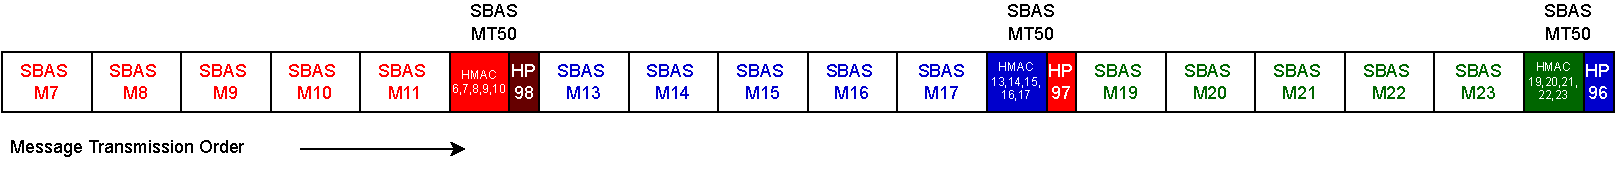
\includegraphics[width=0.5\linewidth]{fig/MT50Schedule.pdf}
\caption{A conceptual diagram of how consecutive MT50 messages relate to each other. The colors correspond to a specific Hash Point along the Hash Path. Each MT50 includes the HMACs of the five previous messages and the Hash Point used for the HMACs sent six messages earlier.}
\label{fig: MT50 Schedule}
\end{figure}

Per the SBAS specifications, in the event of a GNSS integrity alert, an alert message must be sent by Provider four messages in a row.
Therefore,  occasionally an alert message will take priority over an MT50.
The salted Hash Function described below in Equation \eqref{eq: hash path} accommodates small perturbations to the schedule resulting from alert messages, see Section \ref{sec: alert salt}.
Figure \ref{fig: alert schedule} provides a conceptual diagram of how alerts affect the MT50 schedule.
Even with the an MT50 delay, each MT50 must sign the messages it would have signed without an alert.
This is explained in Section \ref{sec: alert salt}.

\begin{figure}
\centering
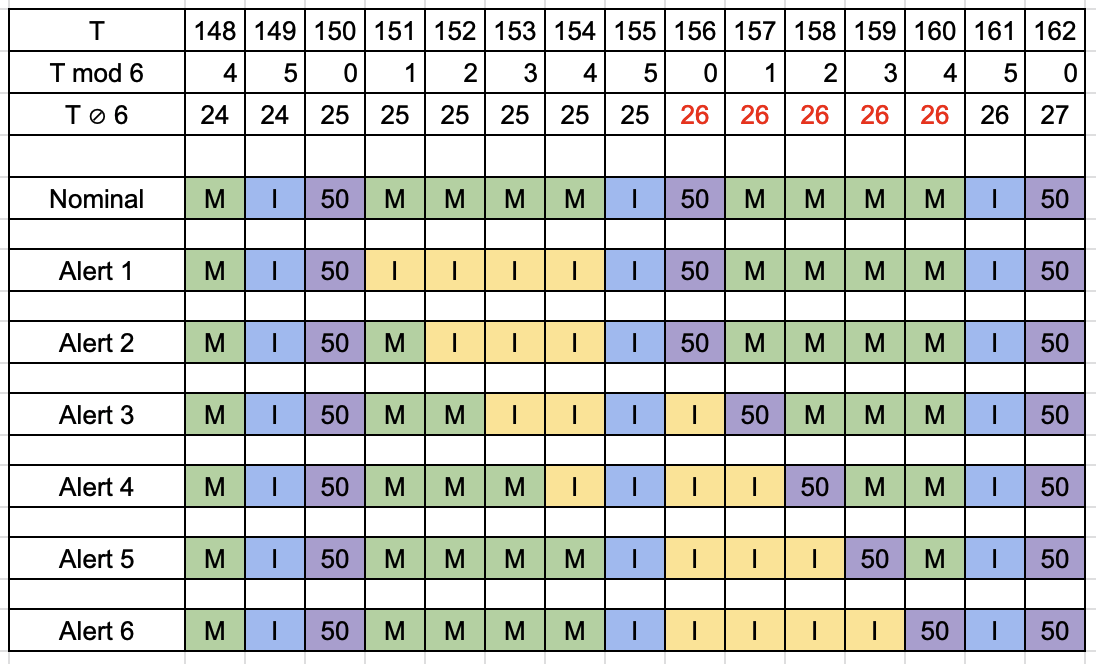
\includegraphics[width=0.5\linewidth]{fig/alertschedule.png}
\caption{Conceptual diagram of how the salting scheme accommodates perturbations to the MT50 schedule. In the diagram, m means a standard message and I means an integrity message. Integrity messages that would be sent on a nominal schedule are marked blue, and extra integrity messages during an alert are marked yellow. Note that $T \oslash 6$ does not change in the event of an alert message MT50 delay, so the Hash Path is preserved. BEAUTIFY ME SO I LOOK LIKE I DIDNT COME FROM EXCEL}
\label{fig: alert schedule}
\end{figure}

\subsection{MT 51}
Table \ref{tab: high-level table} and Table \ref{tab: meta-data table} together provide out proposed definition of MT51 with bit allocations.
To meet requirements specified later, Provider must broadcast MT51 messages approximately every 1 in 18 messages.
These messages do not have to be sent on a rigid schedule and can be sent in the extra space within the current SBAS schedule.

\begin{table}[H]
\center
\begin{tabular}{|c|c|c|c|c|} \hline
	Preamble & MT & Cipher Text Meta Data & Cipher Text & CRC \\ \hline
	4 & 6 & 88 & 128 & 24 \\ \hline
\end{tabular}
\caption{Bit allocation proposed for MT 51 at 250 bits per message. Table \ref{tab: meta-data table} providers greater detail of the ciphertext metadata.}
\label{tab: high-level table}
\end{table}

\begin{table}[H]
\center
\begin{tabular}{|c|c|l|} \hline
	\multicolumn{3}{|c|}{Ciphertext Meta Data} \\ \hline
	Section & Bits & \multicolumn{1}{|c|}{Value} \\ \hline
	Germane SBAS System & 5 & WAAS, EGNOS, BDSBAS, GAGAN, et al. \\ \hline
	\multirow{4}{*}{Germane Key Level} & \multirow{4}{*}{2} & 0 - Spare \\ 
	& & 1 - ECDSA AES key to decrypt Level 1 ECDSA Public Key \\
	& & 2 - ECDSA Level 2 Public Key \\
	& & 3 - TESLA Hash Path End Hash Point \\ \hline
	Germane Key Hash & 16 & Truncated Unsalted 16-bit Hash of Entire Germane Key \\ \hline
	Germane Key Expiration & 29 & GPS Week and Time of Week of Germane Key Expiration \\ \hline
	Authenticating Key Hash & 16 & Truncated Unsalted 16-bit Hash of Entire Authenticating Key \\ \hline
	\multirow{4}{*}{Cipher Text Type} & \multirow{4}{*}{2} & 0 - Public Key, AES Decryption Key, or Hash Path End \\
	& & 1 - Authenticating cipher text derived from the Authenticating Key \\ 
	& & 2 - Spare \\ 
	& & 3 - Spare \\ \hline
	Cipher text Page Number & 4 & The Ordered Section of Germane cipher text - max 16 with 4 bits\\ \hline
	Parity Bit & 1 & Parity bit for a compressed public key \\ \hline
	Spare & 13 & Additional features possible discussed in Section \ref{sec: MT51 modularity} \\ \hline
	Sum Total & 88 & \\ \hline
\end{tabular}
\caption{Bit allocation of ciphertext metadata. To distinguish the key updated with a specific MT51 and the key used to authenticate that MT51, we call the key associated with the MT51-delivered ciphertext the Germane Key and the key used to authenticate that delivered key the Authenticating Key.}
\label{tab: meta-data table}
\end{table}

Our proposed MT51 includes 128 bits of ciphertext and 88 bits of metadata that pertain to how the receiver should interpret that ciphertext.
To distinguish the key updated with a specific MT51 and the key used to authenticate that MT51, we call the key associated with the MT51-delivered ciphertext the Germane Key and the key used to authenticate that delivered key the Authenticating Key.
The metadata specifies the following, matching the order of Table \ref{tab: meta-data table}.
First, the metadata specifies which system the German Key applies to;
second, whether the ciphertext is either an ECDSA public key, an AES decryption key for an ECDSA public key, or a TESLA Hash Path End;
third, a 16-bit hash of the entire Germane Key so that the receiver can immediately associate the ciphertext page with a specific key;
fourth, the expiration time of the Germane Key;
fifth, a 16-bit hash of the entire Authenticating key so that the receiver can immediately associate the ciphertext page with a specific authenticating key;
sixth, whether the payload itself is a key or authentication signature;
seventh, the page number of the ciphertext so that the receiver can piece together all the ciphertext pages over time.

The signatures to authenticate a particular key must derive from the entire set of full MT51 messages used to deliver them.
The metadata associated with a ciphertext includes the expiration time.
These keys are only secure for specific lengths of time, as described in Section \ref{sec: ECDSA Key Structure} and \ref{sec: TESLA Hash Path and HMAC Keys}; hence, the expiration time must be authenticated together with the corresponding ciphertext so that each key is retired securely.
After expiration of a particular key, receivers must reject messages signed with that expired key.

\subsection{Cold Start Procedures}

Upon a receiver startup, a receiver must check that it has a complete set of current, unexpired Level-1 ECDSA public key, Level-2 ECDSA public key, TESLA Hash Path End, and the associated authenticating ciphertext signatures thereof (together, the ``Authentication Stack'').
Without receiving and verifying the entire set of unique MT51s to complete receipt of the Authentication Stack, the receiver cannot assert an authenticated fix, and must ignore the SBAS data derived from the incoming messages.
In any case, Provider repeatedly broadcasts the current Authentication Stack, see Section \ref{sec: MT51 Freq}.
Upon complete receipt of the Authentication Stack, receivers will have to hash the current Hash Point from the recent MT50 to the MT51-provided Hash Path End.
The worst case number of hash computations is the length of the Hash Path and will occur when a receiver turns on near the expiration of the Hash Path.
With receiver standard hardware (e.g., INSERT PROCESSOR HERE), a worst case time of [TIME] happens if the receiver is turned on immediately before a Hash Path expires, which is negligible.
We measured this time by having that processor hash 100,000 times.
In the special case where the receiver has only been off a short time, moving offline and back online during the use of the same Hash Path, the receiver time-of-first-authenticated is just the time required to hash to the Hash Path End.

\section{Methodology} \label{sec: methodology}

\subsection{TESLA Security and Loss Tolerance}

Previous work determined the appropriate security-level lengths under conservative adversary models\cite{Neish_Dissertation}.
That work asserts that a TESLA Hash Point length of 115-bits and an HMAC length of 15-bits is sufficient to deter a super-computer level attack over the time-between-authentication interval and assert a sufficiently low probability of success.
In this work, we round these numbers up to the nearest base-2 number, 128 and 16, respectively.
Increasing these lengths adds additional security-level padding.
The primary reason for 128 Hash Point lengths is that MT51, as specified, has space for 128 bits.
Section \ref{sec: MT51 modularity} discusses why 128 was selected to aid in the scheme's maintenance.
The selection of 16-bit HMAC lengths follows our general strategy of 2-bit lengths, which aids the flexibility of the scheme, as discussed in Section \ref{sec: MT51 modularity}.
The TESLA protocol presents two germane advantages relevant for adoption by SBAS: ciphertext efficiency and loss tolerance.

Regarding authenticating ciphertext efficiency, the overhead required to OTAR a Hash Path does not increase with Hash Path length.
To OTAR a TESLA Hash Path, Provider sends a Hash Path End authenticated with ECDSA.
While a complete OTAR requires a daunting 2048 bits, see Section \ref{sec: MT51 modularity}, the bits do not scale with Hash Path length.
If Provider finds the overhead required to OTAR a Hash Path too burdensome on the schedule, Provider can double the Hash Path's length and halve Hash Path OTAR's frequency.
Increasing the Hash Path length requires Provider to compute a longer Hash Path per OTAR, but this burden is negligible as commodity hardware can compute Hash Paths on the lengths specified in this work in seconds.
At a 128-bit Hash Point length, a Hash Path length on the order of decades is safe from attack \cite{Neish_Dissertation}.

Regarding loss tolerance, TESLA allows receivers to derive past keys lost.
Keys are released backward along Provider's precomputed Hash Path held secret.
Suppose a receiver misses a particular Hash Point; it can derive that missing Hash Point by computing the Hash of the next released Hash Point.
Suppose a receiver misses several day's worths of Hash Points; upon receipt of a new Hash Point, it can Hash all they down to the Hash Path End to assert the new messages' immediate authenticity.
This property scales along the length of the Hash Path.
If a receiver is off longer than the Hash Path's length or applicability, it will need to OTAR the Hash Path End via MT51 and ECDSA.
Each MT50 transmits five HMACS that each separately authenticates a message, rather than a single HMAC that authenticates the five messages together.
This ensures that if a single message is lost, the other four messages' authentication remains unaffected; however, the short 16-bit HMAC length relies on a short time between authentication: in our case, 6-11 seconds.

Our selection of SHA-256 is not necessarily required.
We select SHA-256 because it is standard and widely used.
We select HMAC-SHA-256, which calls SHA-256 as its primitive, to simplify the protocol.
The widespread and straightforward use of SHA-256 aids in the continued security of the scheme.
If the security SHA-256 is broken, it will be widely publicized and quickly deprecated for another hash function.
Providers would simply replace the single function in their implementation and continue operation, much like the recent SHA-1 deprecation.

\subsection{HMAC Security} \label{sec: HMAC security}

For our HMAC use in this scheme to be secure, we must assert there exists no known efficient algorithm that can generate HMAC forgeries.
To meet that, Equation \ref{eq: key} introduces two xor operations on the Hash Point to derive the HMAC keys.
The first is the current time $t_j$.
Without this operation, an adversary can break the security of the scheme.
In the course of SBAS operation, repeated messages occur.
If the HMAC key is not a function of time, then upon receipt of an authenticated message, an adversary can spoof the same message four times in a row until a the next Hash Point comes into effect.
Given the security of HMAC, any bit change among the keys derived from one Hash Point is sufficient to protect against this attack; however, we specify the time of message to aid other aspects of the scheme, see Section \ref{sec: time and keys}.

The second xor operation is the particular SBAS geostationary satellite psuedorandom code (``PRN'').
These codes serve to identify satellites and aid with signal acquisition.
Our use here allows for multiple SBAS geostationary satellites to share the same Hash Path without compromising security.
Without making the HMAC key a function of the broadcasting satellite, upon receipt of an authenticated message, an adversary can spoof the same message as from other satellites.
Once again, any bit change among the keys derived from one Hash Point is sufficient; however, we specify the satellite PRN code for convenience and universal applicability among the SBASs and since they are necessarily unique for each satellite.
While Providers could maintain separate Hash Paths for each satellite, this feature could be used to decrease the time of receipt of the Authentication Stack for cold start receivers.
For instance, WAAS uses three geostationary satellites.
WAAS could use the same Hash Path for of its satellite, and broadcast the set of unique messages that make up the Authentication Stack out of phase, decreasing the time-of-first-authenticated-fix by 66.6\%, while accommodating receivers that do not track each satellite.
Our selection for a single geostationary SBAS satellite time of first fix is discussed in Section \ref{sec: MT51 Freq}.

\subsection{MT51 Modularity} \label{sec: MT51 modularity}

The proposed design of MT51 is fundamentally {\em modular}.
The design of MT51 serves only to deliver pseudorandom data so that its use can be flexible and recycled among different OTAR designs and applications that require delivery of psuedorandom data such as keys, signatures, and Hash Points. 
Its purpose is to deliver large chunks of psuedorandom data to maintain the SBAS authentication scheme and the associated metadata on how the receiver should interpret that ciphertext.
The same message definition delivers TESLA Hash Path Ends, level-2 keys, level-1-key decryption keys, and the authenticating ciphertext required to authenticate each.

Our choice to allow 128-bits per MT51 serves several purposes.
We select 128 and 256-bit security level ECDSA keys there exist standardized, secure elliptic curves those at those security levels, and they are each divisible by 128.
The public keys and derived signatures are twice and four times the security level length, respectively.
These quantities are divisible by 128, meaning that there will be integer numbers of ciphertext pages, and no wasted zero padding will be used to distribute keys.
Table \ref{tab: ciphertext lengths} shows have many messages are required to OTAR each of the key levels.
Our selection could be modified to use the 192-bit level without modifying out scheme, since all of the 192-bit level data is also divisible by 128.
\begin{table}[H]
\center
\begin{tabular}{|c|c|c|c|c|} \hline
	Key Level & Security Level & Public Key Length & OTAR Bit Requirement & MT51s Req. \\ \hline
	    1 & 256 & 512 &  128 & 1 \\ \hline
	    2 & 128 & 256 & 1280 & 10\\ \hline
	TESLA & 128 & 128 &  640 & 5 \\ \hline
\end{tabular}
\caption{Table that delineates the number of MT51s required to complete a single OTAR for a specific key. Level-1 keys require only the 128-bit AES decryption key, hence a single MT51. Level-2 keys require 256-bit key, and 1024 bits of authenticating ciphertext (twice the Level-1 public key length), hence 1280 bits and 10 MT51s. TESLA Hash Path Ends require 128-bit Hash Point and 512 bits of authenticating ciphertext (twice the level-2 public key length), hence 640 bits and 5 MT51s. Each MT51 unique page is required to OTAR.}
\label{tab: ciphertext lengths}
\end{table}

The 128-bit selection supports the modular design.
The design is agnostic to the asymmetric scheme and is recycled for OTAR of the Hash Path Ends, expanding its use to the entire scheme's maintenance, not just the asymmetric portion.
The proposed MT51 standard would require no changes if a more efficient ciphertext efficient scheme (e.g., EC-Schnorr), a quantum-secure scheme, or a different security-level replaced the proposed asymmetric authentication scheme.
The modular design also allows easy expansion of additional features that may desirable to SBAS stakeholders.

Within the ciphertext metadata, we specify the inclusion of a Germane and Authenticating Key hash.
Any identifying feature would suffice, such as the ordered key number, rolling over every $2^{16} = 65536$ keys.
However, the use of hash on the entire key provides additional features.
The key schedule need not be rigid, linear, or sequential.
Provider and ICAO can maintain several redundant level-2 and level-1 keys, respectively, multiple keys, perhaps managed in isolation by Provider and ICAO, for redundant security.
Provider would need to be careful that two unexpired keys don't share the same 16-bit identifying hash; however, this would be a rare event, and Provider would need only randomly draw another key in that event.

To promote service continuity, SBAS Providers could mutually broadcast each other's Hash Path Ends and key maintenance.
SBAS Providers would not need access to each other's secrets; they would only act as a repeater.
Whereas Section \ref{sec: MT51 Freq} discusses higher MT51-frequency to support the local SBAS authentication from cold receiver start, this feature would be low frequency to support the local Provider schedule.
Having Providers broadcasting each other keys at low frequency would aid in the time-of-first-authenticating-fix when transferring to a new SBAS Provider.
Consider two adjacent SBAS systems, such as WAAS and EGNOS, and an aircraft traversing from Europe to North America.
It takes several hours for aircraft to make this journey.
If EGNOS broadcasts the WAAS keys once an hour, any aircraft that makes that journey will receive the keys necessary to operate with WAAS before it enters North America, decreasing the WAAS time of the first authenticated fix to zero. 
At a minimum, SBAS Providers could broadcast adjacent SBAS Providers' keys.
Without this feature, every time an aircraft enters a new SBAS, it essentially enters as a cold-start receiver liable to the amount of time required to get all the ciphertext to start authenticating messages.

Spare bits in the ciphertext metadata could accommodate other features.
These include scheme hyperparameters, such as the choice of a hash function or key or HMAC length.
MT51 messages could authenticate specific messages, identified by 16-bit hashes, immediately with ECDSA.
If keys are ever compromised, MT51 could also disseminate key revocations.
A revocation MT51 would include eight 16-bit hashes of the affected keys and would only need to be broadcast until the keys are retired under standard procedure.
Since each broadcast of an MT51 is accompanied with an germane expiration time, Provider can arbitrarily shorten the applicability of a particular key by rebroadcasting the MT51 with a different expiration time, noting the assumption that receivers actually receive that updated broadcast and that the Hash Path salt may be disrupted since a particular nonce cannot be used more than once, see Section \ref{sec: salt}. 
If Provider can resigns data, the metadata must include a parameter that identifies that particular authentication.
This is because without the germane key hash, authenticating key hash, page number, and authentication instance number, each page of data cannot be associated with each other because they are pseudorandom.
Furthermore, MT51 could manage other authentication schemes, such as an authentication scheme adopted by GNSS.
A GNSS authentication, especially one built on TESLA, would save bandwidth by deferring the GNSS scheme's maintenance to SBAS.

There are many features that can be accommodated by the scheme's modularity; however, if SBAS stakeholders do not want any of these features, then the spare meta bits could also be used to aid in resistance to message loss.
Providers could add redundant HMACS to the MT51 message to redundantly authenticate messages for the event of an MT50 loss.
Moreover, the delivery of 128-bits of authenticating ciphertext could be augmented with fountain codes.
Fountain Codes(1) increase the reliability of delivering MT51 messages and (2) decrease the number of transmitted messages required for an authenticated first fix.
The selection of 128-bits aids in the schemes efficiency since all the data is integrally divisible by 128.
Special care can ensure that using fountain codes in the spare bits to augment those 128-bits would not change the integrally divisible property and maintain efficiency.

\subsection{MT51 Schedule Frequency} \label{sec: MT51 Freq}

As mentioned earlier, we propose that the cryptoperiod of the level-1, level-2, and TESLA Hash Paths be 100, 10, and 1 week, respectively.
Our selections are arbitrary, but any choice must meet security requirements that they are much less than the required exhaustive computational time to break the keys.
Upon cold receiver startup, we desire that the time of the first authenticated fix be reasonably short.
Therefore, Authentication Stack must be sent periodically over their use.
From Table \ref{tab: ciphertext lengths}, a complete Authentication Stack requires 16 MT51s. 
We propose that the current Authentication Stack be transmitted by Provider every 5 minutes so that a cold-start receiver achieves the first authenticated fix in 5 minutes, assuming no message loss.
This requirement would require that a message from the set of 16 unique MT51s be transmitted 1 out of every 18 messages, rounded up.
With multiple geostationary satellites, the satellites can broadcast the unique MT51s out of phase to decrease the authenticated first fix time.

Furthermore, the next keys, applicable immediately upon expiration of the current keys must be sent well before their actual use for a seamless transition as keys expire.
To protect a specific new key's security, it would be prudent to only send that new key just before use.
For instance, we suggest Provider send the next 100-week level-1 key repeatedly beginning five weeks before its actual use and send the next 10-week level-2 and 1-week TESLA Hash Path End 1 week before its actual use.
To show how little this consideration affects the MT51 SBAS bandwidth, if a Provider sent the next Authentication Stack once every hour, together with the current Authentication Stack once every 5 minutes, Provider would need to send a message from the set of 32 unique MT51s 1 out of every 17 messages, rounded up.

We note that is it not actually required that Provider and receivers stick to a set schedule for the key periods nor the Hash Paths.
As discussed before, the MT51 metadata and modularity affords flexibility in expirations of particular keys and the agreed schedule for expirations.
Moreover, switching Hash Paths by Provider without warning does not add computational complexity to receiver verification.
Each Hash Point is a hash, and hashes have constant-time look-up computational complexity.
This means if Provider were to switch Hash Paths without warning, receiver would need only one additional computation to check that the new Hash Point is the preimage to another ECDSA-verified Hash Path End.
This means that SBAS could incorporate unscheduled or stochastic Hash Path switches, provided the appropriate MT51s are sent in advance noting that the MT51s only specify Hash Path End expirations and not their actual use time.
If stakeholders elect not to have a rigid Hash Path schedule, a maximum Hash Path length upper bound must be specified so that receivers do not get stuck in an infinite hashing loop attempting to hash back down to an ECDSA-authenticated Hash Path End.

\subsection{TESLA Hash Path Salt} \label{sec: salt}

The security of each TESLA Hash Path hinges on the difficulty of computing any earlier preimage Hash Point of the Hash Path before Provider releases it.
Unsalted Hash Paths are susceptible to precomputation attacks, also known as the Rainbow Table Attack.
An attacker precomputes a large number of Hash Paths and stores them hoping that one of those precomputed Hash Paths contains the currently secure Hash Point mid Hash Path.
If that ever occurs, the attacker then has in-memory Hash Points earlier on the no-longer-secure Hash Path and can therefore spoof SBAS authenticated messages.
To prevent this, we must introduce random variations called salt to the Hash Function that make a precomputation attack infeasible.

In designing a salt scheme, we desire the following characteristics.
First, the salt scheme must be sufficient to deter precomputation attacks.
Second, the scheme must accommodate spontaneous and episodic message loss by the receiver (e.g., receiver interference, receiver offline cold start).
Third, the scheme must not pose a burden on the message scheduler.
A 128-bit salt would suffice the security requirements.
Given the modular design of the proposed MT51, one could append to the metadata definitions of Table \ref{tab: meta-data table} a designation for the salt of a particular Hash Path.
This would require an additional message sent to OTAR a Hash Path, which would likely not pose too much of a burden on the SBAS schedule.
However, we propose that the Hash Path salt derives from the level-2 signature protocol, thereby saving a message.
From Equation \eqref{eq: hash path}, we propose Provider compute a Hash Path Salt $S^P$ via Algorithm \ref{alg: salt}.

\begin{algorithm}[H] \label{alg: salt}
\SetAlgoLined
{\bf Provider} \\
Provider generates cryptographically-secure nonce $K$;\\
With elliptic curve base point $G$, Provider computes elliptic curve point $C = K \times G$; \\
$S^P = H(C)$; \\
Provider computes hash path $p^P_1 ... p^P_n$ with Equation \eqref{eq: hash path}; \\
Provider generates ECDSA signature of $p^P_n$ with $C$ and broadcasts before actual use of Hath Path; \\
{\bf Receiver} \\
Receiver receives $p^P_n$ with ECDSA signature for authentication; \\
Receiver derives $C$ from ECDSA signature; \\
$S^P = H(C)$; \\
Receiver authenticates new message on a new Hash Path upon receipt of $p^P_{n-1}$.
\caption{Transmitting Salt $S^P$ without additional message with ECDSA}
\end{algorithm}

With every ECDSA signature, Provider computes a cryptographically secure nonce.
With Algorithm \ref{alg: salt}, the salt derives from a public quantity derived from this nonce.
For ECDSA, this is the curve point $C$ (Wikipedia notation), and for EC-Schnorr signatures, this is $r$ (Wikipedia notation).
This $C$ is cryptographically-secure random since it derives from the cryptographically-secure nonce generated at signing; using it as the Hash Path salt compromises neither the signing key nor the Hash Path  and saves an MT51 OTAR message.

While this scheme poses the advantage of one less message to OTAR, it hinders the flexibility of the scheme.
Using a nonce more than once reveals the secret key used to authenticate the data.
This means, that the Hash Path and its authentication signatures are immutable.
Provider cannot resign a Hash Point mid Hash Path to save receivers the computation of hashing down to the signed Hash Path End because the salt derived therefrom would be different.
Providers cannot change any of the meta data (e.g., the expiration time) either.
To reincorporate these two features, as mentioned above, Provider could distribute the salt as a separate MT51.

\subsection{Loss Tolerant TESLA Counter} \label{sec: alert salt}

In the standard TESLA formulation, the Hash Function uses the integer denoting the number of Hash Path Hash Points from the Hash Path start.
We propose using an analog: the integer time of message sending and arrival time.
Sending and arrival times, rounded down to the nearest integer, are the same for Provider and receiver, respectively, since messages are sent each second and transmission time-of-flight is less than a second.
Using the time, instead of the integer number of points from path start, provides several advantages.
Upon start, a receiver knows how to verify a Hash Point, since Equation \eqref{eq: hash path} is only a function of current integer time and the ECDSA authenticating ciphertext.
Moreover, it allows the switching of Hash Paths to occur on a non-rigid schedule.
While we specify a week interval, and it would be natural to have a new Hash Path begin at the beginning of a GNSS week, Provider need not communicate the start and length of Hash Paths as overhead or metadata for a non-rigid schedule because of the hashing properties of the Hash Point.
If Provider were to arbitrarily switch Hash Paths, there is a constant-time complexity for the receiver to check if a new Hash Point hashes to the current Hash Path or a new one.

While in standard operation, Provider will send an MT50 every six seconds.
However, the SBAS alert requirements specify that, upon an alert, alert messages must be sent immediately for four consecutive seconds.
Since Provider computes the entire Hash Path before its use, including assuming the $t_i$'s associated with each Hash Point, alerts will interfere with the six-second MT50 schedule, and TESLA counter proposed.
To accommodate perturbations of the authentication schedule, we propose (1) nominally sending each MT50s when $t_i \mod 6 = 0$ and (2) performing an integer division of 6 on the time $t_i$.
If an alert occurs, requiring four consecutive messages that displaces a TESLA authentication between one and four seconds after $t_i \mod 6 = 0$, the Hash Path is preserved because $t_i \oslash 6 = (t_i + 4) \oslash 6$ when $t_i \mod 6 \leq 4 $.
Figure \ref{fig: alert schedule} provides a conceptual diagram of how the TESLA counter is preserved in the event of alert messages.

To assert the security of our scheme, it is essential that, in the event of an alert, that any delayed MT50 sign the original messages corresponding to the loosely-synchronized schedule.
Concretely, in Figure \ref{fig: alert schedule} in the row labeled Alert 6, (1) the MT50 of column 160 must sign the messages of columns 151 through 155, (2) the MT 50 of column 162 must sign the messages of columns 157 through 161, and (3) the message of column 156 remain unauthenticated.
For the rows labeled alerts 3 through 6, the integrity messages of column 156 each remain unauthenticated.
This is acceptable because those messages will only tell receivers not to use the service, and the surrounding integrity messages will be authenticated anyway.
Without asserting this requirement, this security scheme becomes less secure.
The security hinges on the loosely-synchronized schedule, which is susceptible to a replay attack.
If authenticated messages are occasionally sent after their agreed schedule, then the amount of replay delay required is occasionally reduced and an adversary could spoof alerts to make such a replay attack easier.

\subsection{Use of Time in Hash Path} \label{sec: time and keys}

The TESLA protocol assumes that Provider and receiver are loosely time-synchronized.
To break the TESLA protocol's security, an attacker must hack the receiver time so that its time is 6 seconds behind Provider time.
In the above formulations, we proposed including the times $t_i$ and $t_j$ in the TESLA counter and Hash Point to key derivations.
As proposed, if Provider and the receiver are not time-synchronized within 1-second, the authentication scheme fails to certify messages as authenticated since all the keys derive from the integer time in seconds.
This helps make SBAS message spoofing more complex by requiring that any SBAS spoofer also spoof the GNSS time.

\subsection{Future Proofing}

As already mentioned, MT50 and MT51 are agnostic to the asymmetric cryptographic security scheme and hash function primitives.
When the security of a primitive becomes compromised, the SBAS MT scheme need not change.
Providers and receivers will have to change the primitives used separately.
Since MT51 provides 128-bits of ciphertext per message, and standardized cryptographic primitive lengths are, generally, integer factors of 128, changes to the scheme would increase or decrease the number of pages required to transmit information.
If the security of the 128-bit truncated SHA-256 is every compromised, SBAS could double the Hash Point length space without affecting the MT50 frequency as follows.
Suppose the Hash Point space is the set of 256-bit integers, like the untruncated SHA-256.
Each MT50 will transmit half of a Hash Point, and each HMAC key will derive from two consecutive MT50 messages.
This increases the time-between authentication by a few seconds; however, it doubles the Hash Path security and maintains the loss-tolerant properties.

\pagebreak

\section{Full Stack Simulation and KPIs}

\begin{itemize}
	\item Discuss methodology of monte-carlo simulation
	\item Discuss Figure \ref{fig:time-of-first-fix-mc}
	\item Availability
	\item Continuity
\end{itemize}

\begin{figure}[H]
	\centering
	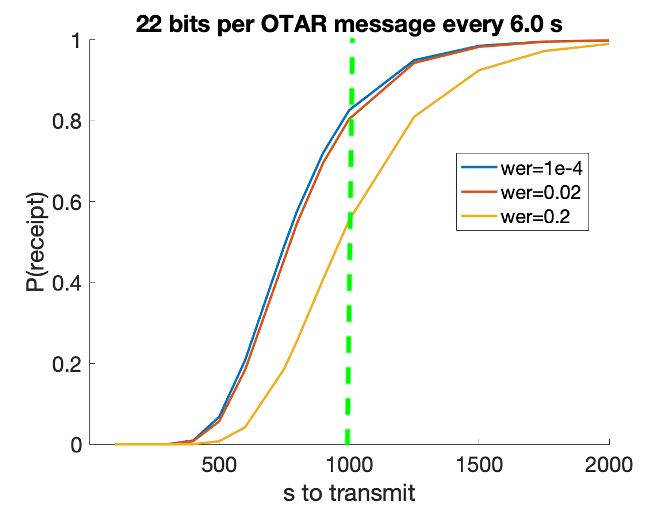
\includegraphics[width=0.4\linewidth]{fig/integrated_mc.png}
	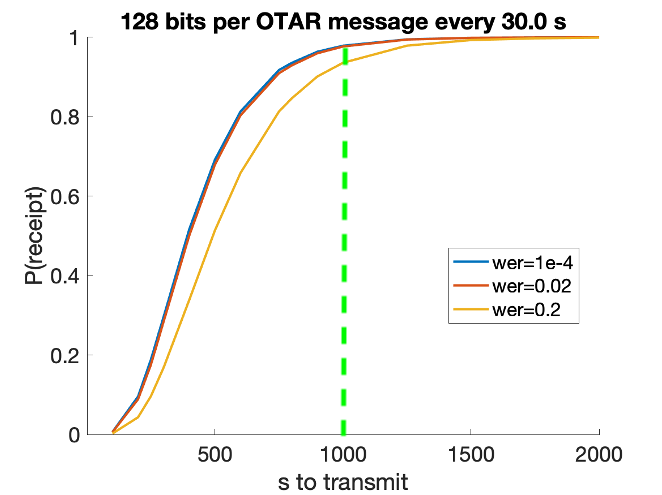
\includegraphics[width=0.4\linewidth]{fig/modular_mc.png}
	\caption{Comparison of time-of-first-fix of spare-bit approach (left) and modular approach (right) via monte carlo methods.}
	\label{fig:time-of-first-fix-mc}
\end{figure}

\section{Loose-time Synchronization and Operational Procedures}

\subsection{TESLA Timing Synchronization and Replay Attacks}
\begin{itemize}
	\item How TESLA requires time sync and therefore SBAS is vulnerable
	\item The worst Replay Attack
\end{itemize}

\subsection{Time Sync Option A: Reliance on external connection}

To verify that the timing hasn't been hacked
\begin{itemize}
	\item Discussion of allowing external connection
	\item Discussion of allowing only {\em external broadcast} connection
\end{itemize}

\subsection{Option B: Reliance on exclusive receiver clock}

Primary reference \cite{time_sync_paper}

To verify that the timing hasn't been hacked
\begin{itemize}
	\item Minimum calibration requirement given clock drift and GPS and SBAS time sync fusion
	\item machine state time procedures
	\item tie to periodic maintenance
\end{itemize}

\section{Remaining Work}

Scheme extendable to any broadcast only connection (e.g., having traffic lights broadcast their state (e.g., red, green) without spoofing problem)

\section*{Alternative Design}

\begin{table}[H]
\center
\begin{tabular}{|c|c|c|c|c|} \hline
	Preamble & MT & Cipher Text Meta Data & Cipher Text & CRC \\ \hline
	4 & 6 & 24 & 192 & 24 \\ \hline
\end{tabular}
\caption{Bit allocation proposed for MT 51 at 250 bits per message. Table \ref{tab: meta-data table} providers greater detail of the ciphertext metadata.}
\label{tab: high-level table1}
\end{table}

\begin{table}[H]
\center
\begin{tabular}{|c|c|l|} \hline
	\multicolumn{3}{|c|}{Ciphertext Meta Data} \\ \hline
	Section & Bits & \multicolumn{1}{|c|}{Value} \\ \hline
	\multirow{4}{*}{Germane Key Level} & \multirow{4}{*}{2} & 0 - Spare \\ 
	& & 1 - ECDSA AES key to decrypt Level 1 ECDSA Public Key \\
	& & 2 - ECDSA Level 2 Public Key \\
	& & 3 - TESLA Hash Path End Hash Point \\ \hline
	Germane Key Expiration & 10 & GPS Week and Time of Week of Germane Key Expiration \\ \hline
	\multirow{4}{*}{Cipher Text Type} & \multirow{4}{*}{2} & 0 - Public Key, AES Decryption Key, or Hash Point Root \\
	& & 1 - Authenticating cipher text derived from the Authenticating Key \\ 
	& & 2 - Spare \\ 
	& & 3 - Spare \\ \hline
	Cipher text Page Number & 4 & The Ordered Section of Germane cipher text - max 16 with 4 bits\\ \hline
	Next or Current Key & 1 & Either next key or current key \\ \hline
	Spare & 5 & \\ \hline
	Sum Total & 24 & \\ \hline
\end{tabular}
\caption{Bit allocation of ciphertext metadata. To distinguish the key updated with a specific MT51 and the key used to authenticate that MT51, we call the key associated with the MT51-delivered ciphertext the Germane Key and the key used to authenticate that delivered key the Authenticating Key.}
\label{tab: meta-data table1}
\end{table}

\bibliographystyle{ieeetr}
\bibliography{references}

\end{document}
